\documentclass{acm_proc_article-sp}
\usepackage{amsmath}

\begin{document}

\title{A Novel Similarity-Search method for Mathematical \\ Content in {\ttlit LaTeX} Markup}

\numberofauthors{2} 
\author{
\alignauthor Wei Zhong,\; Hui Fang\\
       \affaddr{Dept. of Electrical and Computer Engineering}\\
       \affaddr{University of Delaware}\\
       \affaddr{Newark, DE USA}\\
       \email{\{zhongwei, hfang\}@udel.edu}
}

\maketitle
\begin{abstract}
A relaxed structural matching search method, along with a symbolic similarity measurement algorithm for mathematical content search is proposed. 
Our approach uses an intermediate tree representation to capture structural information of mathematical expression, and based on a previous idea which indexes math expression structure through tree leaf-root paths, we further describe an advanced AND search method in a formal way. This search method can be used to test query/document subexpression isomorphism or evaluate the symbolic similarity between math expressions with consideration of their $\alpha$-equivalence. 
For the purpose of evaluation, we also implement a search engine based on our idea. 
\end{abstract}

\category{H.3}{Information Search and Retrieval}{Miscellaneous}
\terms{Algorithms}

\keywords{mathematical searching, language processing, search engine}

\section{Introduction}
With \textit{MathJax} becoming popular, more and more \LaTeX{} markups can be crawled directly from many websites. 
In order to search those mathematical language in \LaTeX{} markups, a search method that can respect the properties of math expression needs to be developed. 
Although many researches have been conducted to retrieve information in structured content (e.g. \textit{MathML}), information retrieval on \LaTeX{} math content is still not well-studied or exhaustively covered by mainstream IR research, compared to that on general text.

Unlike general text content, mathematical language, by its nature, has many differences from other textual documents, there are a number of new problems in measuring mathematical expression similarity.
Among those problems, we know one math expression can be transformed to alternative forms, e.g. $\frac{a + b}{c}$ and $\frac{a}{c} + \frac{b}{c}$ should be considered as semantically identical. To identify those variations requires search engine to apply mathematical transformation rules to a query in order to obtain all forms of relevant expressions. 
Further, math expressions with the same evaluated value may also be considered relevant, in this case, $\sin(\frac {\pi} 2)$ and $1$ are equivalent. Some computational search engines (e.g. \textit{Symbolab} and \textit{WolframAlpha}) are aware of these problems.
But sometimes we need to rely on conventions and context to distinguish expressions such as $f(a+b)$ and $c(a+b)$, because the symbol $f$ in the former expression is likely to represent function instead of a variable, 
in addition, expression such as $f^{-1}$ can either be reciprocal or an inverse function.
Moreover, a higher level of understanding of mathematic knowledge may be required for math-aware search engine to find the results for queries such as ``find an article related to the four color theorem" (from NTCIR-10 Math topics~\cite{ntcirtopic}).

Yet the problems addressed above are not considered in this paper, instead, we are focusing on the aspects which does not require a ``good understanding" of mathematics, we target our research domain to be the following:
The first is structural similarity. For example, $ax+(b+c)$ is not equivalent to $(a+b)x+c$ although they have the same set of symbols, this is because their structural difference. However, as the position of operands in math expression can be commutative in some cases, structural similarity is often measured by substructure isomorphism if we use operation tree~\cite{goodsurvey} to represent math expressions.
The second is symbolic similarity, with the consideration of $\alpha$-equivalence. We know that symbols can be used interchangeably in each math formula to express the same meaning, e.g. $a^2+b^2=c^2$ and $x^2+y^2=z^2$. Nevertheless, we still weight symbolic similarity sometimes, for instance, $E=mc^2$ is considered more meaningful when exact symbols are used rather than just being structurally identical with $y=ax^2$.
On the other hand, we should also weight $\alpha$-equivalent expressions more, that is, changes of symbols in expression preserve more syntactic similarity when changes are made by substitution, e.g. for query $x(1+x)$, expression $a(1+a)$ are considered more relevant than $a(1+b)$. Because the ``bond variable" $x$ and $a$ here are at the same positions and both supposed to represent the same value.
All the points addressed here makes transitional IR methods (e.g. bag of words model and tf-idf weighting) deficient to handle math content. 

\section{Related Work}
Similarity/boolean search for mathematical content is not a new topic,
conference in this topic is getting increasingly research attention and the proposed systems have progressed considerably~\cite{ov}.
DLMF project from NIST~\cite{Youssef03,Youssef05} and MIaS system~\cite{mias11a,mias11,mias:thesis}, notably, use text-based approaches and utilize existing models to deal with math content on top of existing IR tools (such as \textit{Apache Lucene}). 
They are commonly using augmentation and normalization (by ordering the subexpressions) to enumerate and represent all possible sequences of commutative operands.
However, augmentation usually requires to index combination of both symbols (e.g. $a$ and $b$) and unified items (\textit{id}, \textit{const}) in different levels of math expression, thus implies inefficient storage space usage for complex expressions.
MWS~\cite{Kohlhase06,Kohlhase0p4,Kohlhase0p5} takes a \textit{automatic theorem proving} approach and uses \textit{term indexing}~\cite{graf96} to minimize the cost of unification algorithm which is able to find if two expressions are equivalent. However, their index relies on RAM memory and consumes a considerable space~\cite{Kohlhase0p5}, and it indexes all sub-terms of a formula~\cite{Kohlhase06}.

\begin{figure}
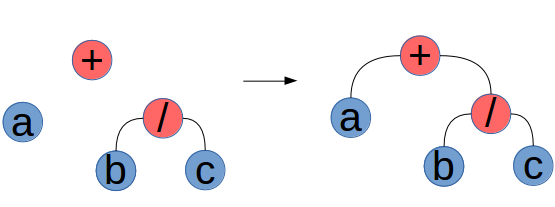
\epsfig{file=attach.png, height=1.2in, width=3in}
\caption{Example of Sub-tree generation for the addition grammar.}
\end{figure}

\bibliographystyle{unsrt}
\bibliography{sigproc}  % sigproc.bib is the name of the Bibliography in this case

\end{document}
